\documentclass[border=3pt]{standalone}
% Shared preamble for every generated figure.
% Matches the report: newtx (Times), greyscale, square boxes.
\usepackage{newtxtext,newtxmath}
% newtx's typewriter (txtt) draws a slashed zero; use Latin Modern instead.
\renewcommand{\ttdefault}{lmtt}
\usepackage{tikz}
\usetikzlibrary{positioning,arrows.meta,calc,fit,backgrounds,shapes.geometric,
                decorations.pathreplacing,decorations.pathmorphing,matrix,patterns}

\definecolor{figgrey}{gray}{0.88}
\definecolor{figmid}{gray}{0.60}
\definecolor{figdark}{gray}{0.35}

\tikzset{
  fig/.style={font=\small},
  box/.style={draw,thick,minimum height=8mm,minimum width=22mm,align=center,
              inner sep=2pt,font=\small},
  greybox/.style={box,fill=figgrey},
  smallbox/.style={draw,minimum height=6mm,minimum width=16mm,align=center,
                   inner sep=2pt,font=\scriptsize},
  ln/.style={-{Stealth[length=2.2mm,width=1.8mm]},thick},
  lnb/.style={{Stealth[length=2.2mm,width=1.8mm]}-{Stealth[length=2.2mm,width=1.8mm]},thick},
  lbl/.style={font=\scriptsize,inner sep=1.5pt},
  note/.style={font=\scriptsize\itshape,inner sep=1.5pt},
}

\begin{document}
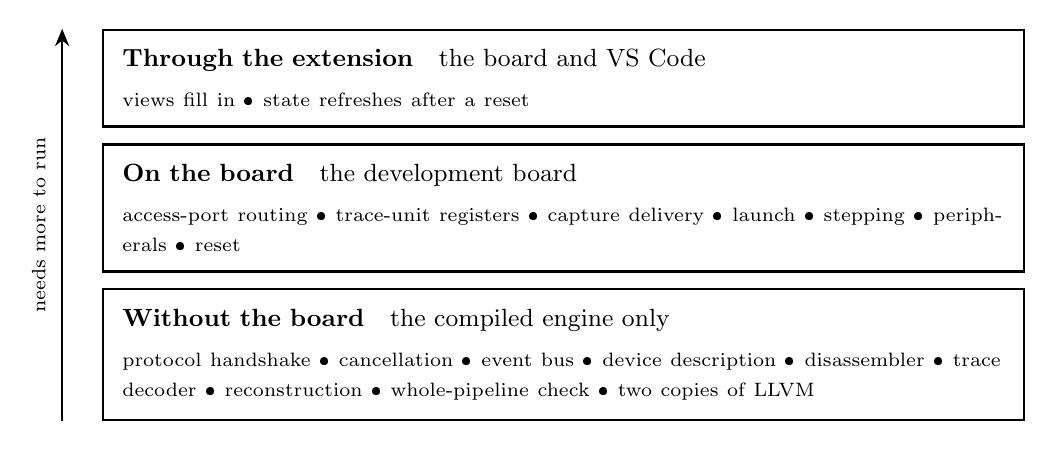
\begin{tikzpicture}[fig,
  grp/.style={draw,thick,text width=112mm,align=left,inner sep=2.5mm}]
\node[grp] (t3) {\textbf{Without the board}\quad the compiled engine only\\[1.2mm]
  {\scriptsize protocol handshake \textbullet\ cancellation \textbullet\ event bus \textbullet\ device description \textbullet\ disassembler \textbullet\ trace decoder \textbullet\ reconstruction \textbullet\ whole-pipeline check \textbullet\ two copies of LLVM}};
\node[grp,above=2mm of t3] (t2) {\textbf{On the board}\quad the development board\\[1.2mm]
  {\scriptsize access-port routing \textbullet\ trace-unit registers \textbullet\ capture delivery \textbullet\ launch \textbullet\ stepping \textbullet\ peripherals \textbullet\ reset}};
\node[grp,above=2mm of t2] (t1) {\textbf{Through the extension}\quad the board and VS Code\\[1.2mm]
  {\scriptsize views fill in \textbullet\ state refreshes after a reset}};
\draw[ln] ($(t3.south west)+(-5mm,0)$) -- ($(t1.north west)+(-5mm,0)$);
\node[lbl,rotate=90] at ($(t3.south west)!0.5!(t1.north west)+(-8mm,0)$) {needs more to run};
\end{tikzpicture}
\end{document}
